\documentclass[11pt, border=3pt]{standalone}
\usepackage{fontspec}\usepackage{unicode-math}
\setsansfont{Fira Sans}[UprightFont=*-Light, BoldFont=*-SemiBold]
\setmathfont{Fira Math}\renewcommand{\familydefault}{\sfdefault}
\usepackage{tikz}\usetikzlibrary{arrows.meta, calc}
\definecolor{nuit}{HTML}{3E2A57}\definecolor{gris}{HTML}{8A8F98}
\definecolor{violet}{HTML}{800080}\definecolor{vert}{HTML}{00AA44}
\def\pas{99}
\def\only<#1->#2{\ifnum#1>\pas\relax\else#2\fi}
\begin{document}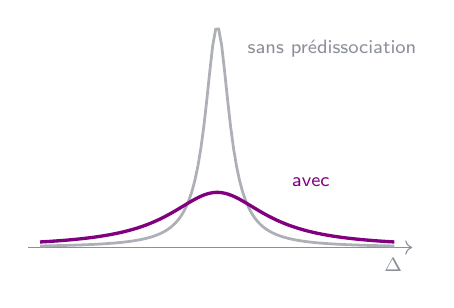
\begin{tikzpicture}[x=0.75cm, y=1.1cm]
        \draw[gris, ->] (-3.2,0) -- (3.3,0) node[below left, font=\scriptsize] {$\Delta$};
        \draw[gris!70, line width=1pt, domain=-3:3, samples=120] plot (\x, {2*0.25/(\x*\x + 0.0625)/3.1416});
        \draw[violet, line width=1.2pt, domain=-3:3, samples=120] plot (\x, {2*1/(\x*\x + 1)/3.1416});
        \node[gris, font=\scriptsize, anchor=west] at (0.35,2.3) {sans prédissociation};
        \node[violet, font=\scriptsize, anchor=west] at (1.1,0.75) {avec};
      \end{tikzpicture}\end{document}
